\documentclass{beamer}
\usepackage[utf8]{inputenc}
\usepackage{hyperref}
\usepackage{multicol}
\usepackage{hyperref}
\usepackage{amsmath}
\usepackage[english]{babel}
\usepackage{algorithm}
\usepackage[noend]{algpseudocode}

\inputencoding{utf8}

\mode<presentation> {
    \usetheme{Madrid}
}

\usepackage{graphicx}
\usepackage{booktabs}

\title[Dinamica]{Programaci\'on Dinamica}
\author{Ernesto Rodriguez - Juan Roberto Alvaro Saravia}
\institute{
    Universidad Francisco Marroquin \\
    \medskip \textit{ernestorodriguez@ufm.edu - juanalvarado@ufm.edu}
}

\date[\today]{}

\begin{document}

\begin{frame}
\titlepage
\end{frame}


\begin{frame}
    \frametitle{Programaci\'on Dinamica}
    \begin{itemize}
        \item{Consiste en dividir el problema en instancias m\'as simples
        y resolverlas recursivamente}
        \item{Similar a divide and conquer}
        \item{Sin embargo, aplica cuando el mismo sub-problema debe ser
        resuelto varias veces}
        \item{{\bf Idea:} Almacenar soluciones que ya hayan sido
        calculadas para evitar tener que calcularlas nuevamente.}
        \item{Se utiliza a menudo en problemas de optimizaci\'on}
    \end{itemize}
\end{frame}

\begin{frame}
    \frametitle{Ejemplo: Secuencia de Fibonacci}
\end{frame}

\begin{frame}
    \frametitle{Ejemplo: Secuencia de Fibonacci}
    \begin{algorithm}[H]
        \caption{Fibonacci}
        \begin{algorithmic}[1]
        \Procedure{Fibonacci}{$n$}
        \If{$n\equiv 0$}
        \State{$\mathtt{return}\ 0$}
        \EndIf
        \If{$n\equiv 1$}
        \State{$\mathtt{return}\ 1$}
        \EndIf
        \State{$\mathtt{return}\ \mathtt{Fibonacci}(n-1)+\mathtt{Fibonacci}(n-2)$}
        \EndProcedure
        \end{algorithmic}
    \end{algorithm}
\begin{itemize}
    \item{¿Cual es la complejidad respecto a $n$ de este algoritmo?}
    \item{¿Por que es tan lento?}
    \item{¿Que trabajo estamos repitiendo?}
    \item{¿Podemos optimizar?}
\end{itemize}

\end{frame}

\begin{frame}
\frametitle{Mejorando la funci\'on de Fibonacci}
\begin{itemize}
    \item{Consideremos la aplicaci\'on recursiva: $\mathtt{Fibonacci}(n-1)+\mathtt{Fibonacci}(n-2)$
    \begin{itemize}
        \item{Ambos casos deben llamar $\mathtt{Fibonacci}(n-3)$, $\mathtt{Fibonacci}(n-4)$, ect}
        \item{Cada llamada recursiva crea un arbol de ejecici\'on que repite el trabajo que ya
        fue hecho}
    \end{itemize}
    }
    \item{Estamos repitiendo cantidades excesivas de trabajo, en efecto, tiene
    un crecimiento exponencial el arbol de ejecuci\'on}
    \item{{\bf Idea:} Guardemos el trabajo que ya haya sido llevado a cabo, asi
    evitamos repetir nuestros pasos}
\end{itemize}
\end{frame}

\begin{frame}
\frametitle{Fibonacci mejorado}
\end{frame}

\begin{frame}
    \frametitle{Fibonacci mejorado}
    \begin{algorithm}[H]
        \caption{FibonacciLineal}
        \begin{algorithmic}[1]
        \Procedure{FibonacciLineal}{$n$}
        \State{$\mathtt{let}\ cache\gets\mathtt{int}[n+1]$}
        \State{$cache[0]\gets 0$}
        \State{$cache[1]\gets 1$}
        \For{$\mathtt{let}\ i=2$ {\bf upto} $n$}
            \State{$cache[i]\gets cache[i-1]+cache[i-2]$}
        \EndFor
        \State{$\mathtt{return}\ cache[n]$}
        \EndProcedure
        \end{algorithmic}
    \end{algorithm}

    \begin{itemize}
        \item{¿Cual es la complejidad respecto a $n$?}
    \end{itemize}    

\end{frame}

\begin{frame}
\frametitle{Programaci\'on Dinamica}
Por lo general, se utiliza el siguiente proceso:
\begin{itemize}
    \item{Caracterizar la estructura de una soluci\'on optima}
    \item{Definir recursivamente el valor de cada pedazo de la soluci\'on}
    \item{Calcular recursivamente cada valor, por lo general de abajo hacia arriba}
    \item{Recuperar la soluci\'on final de la estructura que fue construida}
\end{itemize}
\end{frame}

\begin{frame}
\frametitle{Corte de Barras}
Problema:
\begin{itemize}
    \item{Una empresa compra barras de acero y los corta en secciones
    m\'as peque\~nas}
    \item{Cada corte es gratuito}
    \item{La empresa quiere optimizar ganancias: Cortar las barras de acero
    de tal forma que las barras resultantes se puedan vender al mejor precio}
    \item{Las barras se cortan en intervalos enteros}
\end{itemize}
A continuaci\'on se muestra la tabla de precios de cada segmento de acero:
\begin{center}
    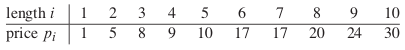
\includegraphics[width=10cm]{precios.png}
\end{center}
\end{frame}

\begin{frame}
\frametitle{Caracterizaci\'on del problema}
\begin{itemize}
    \item{¿Cuantas possibles combinaciones puede cortarse una barra de longitud $l$?}
    \item{¿Es factible explorar todas las combinaciones para encontrar una soluci\'on optima?}
    \item{¿Es necesario considerar todas las posibles combinaciones para encontrar una
    soluci\'on optima?}
\end{itemize}
\end{frame}

\begin{frame}
\frametitle{Planteamiento del Problema}
\begin{itemize}
    \item{Se utilizaran sumas para denotar cortes: $l=i_0 + i_1 + \ldots + i$, por
    ejemplo, $7=2+2+4$ corresponde a una barra de longitud $7$ que fue cortado en
    segmentos de $2$, $2$ y $4$}
    \item{El objetivo es buscar la combinaci\'on de cortes: $r_n=\mathtt{max}(p_n,r_1+r_{n-1},
    r_2+r_{n-2},\ldots,r_{n-1}+r_1)$
    \begin{itemize}
        \item{Esto corresponde a hacer un corte inicial $r_i$ y a eso agregar recursivamente
        los cortes restantes $r_n$}
        \item{La idea es optimizar cada uno de los pasos en el proceso de cortado}
    \end{itemize}
    }
\end{itemize}
\end{frame}

\begin{frame}
    \frametitle{Primer intento}
\end{frame}    

\begin{frame}
    \frametitle{Primer intento}
    \begin{algorithm}[H]
        \caption{Cortar}
        \begin{algorithmic}[1]
        \Procedure{Cortar}{$p,l$}
        \If{$n\equiv 0$}
        \State{$\mathtt{return}\ 0$}
        \EndIf
        \State{$\mathtt{let}\ q\gets -\infty$}
        \For{$\mathtt{let}\ i=0$ {\bf to} $l$}
        \State{$q\gets \mathtt{max}(q,p[i]+\mathtt{Cortar}(p,n-i)$}
        \EndFor
        \State{$\mathtt{return}\ q$}
        \EndProcedure
        \end{algorithmic}
    \end{algorithm}

    \begin{itemize}
        \item{¿Cual es la complejidad del algoritmo?}
    \end{itemize}
    \end{frame}

\begin{frame}
\frametitle{Segundo intento}
\begin{itemize}
\item{Crear un arreglo}
\item{Cada vez que se encuentra una soluci\'on, almacenarla en el arreglo}
\item{De esa manera, se evita tener que calcular multiples veces la misma soluci\'on}
\item{Simplemente consiste en modificar el algoritmo que ya existe con un arreglo
dise\~nado para guardar soluciones intermedias}
\end{itemize}
\end{frame}

\begin{frame}
\frametitle{Segundo intento}
\end{frame}

\begin{frame}
    \frametitle{Segundo intento}
    \begin{algorithm}[H]
        \caption{CortarMemorizado}
        \begin{algorithmic}[1]
        \Procedure{CortarMemorizado}{$p,l$}
        \State{$\mathtt{let}\ res\gets\mathtt{int}[l+1]$}
        \For{$\mathtt{let}\ i\gets 0$ {\bf upto} $l$}
            \State{$res[i]\gets -\infty$}
        \EndFor
        \State{$\mathtt{return}\ \mathtt{CortarMemorizadoAux}(p,l,res)$}
        \EndProcedure
        \end{algorithmic}
    \end{algorithm}
\end{frame}

\begin{frame}
    \frametitle{Segundo intento}
    \begin{algorithm}[H]
        \caption{CortarMemorizadoAux}
        \begin{algorithmic}[1]
        \Procedure{CortarMemorizadoAux}{$p,l,res$}
        \If{$res[l]\geq 0$}
        \State{$\mathtt{return}\ res[l]$}
        \EndIf
        \State{$\mathtt{let}\ q\gets -\infty$}
        \If{$n\equiv 0$}
        \State{$q\gets 0$}
        \Else
        \For{$i\gets 1$ {\bf to} $n$}
        \State{$q\gets \mathtt{max}(q,p[i]+\mathtt{CortarMemorizadoAux}(p,n-i,res))$}
        \EndFor
        \EndIf
        \State{$r[n]\gets q$}
        \State{$\mathtt{return}\ q$}
        \EndProcedure
        \end{algorithmic}
    \end{algorithm}
    ¿Podemos eliminar la recursion?
\end{frame}

\begin{frame}
    \begin{center}
    
\includegraphics[width=6cm]{wecan.jpg}
    \end{center}
\end{frame}

\begin{frame}
\frametitle{Tercer intento}
\end{frame}

\begin{frame}
\frametitle{Tercer intento}

\begin{algorithm}[H]
    \caption{CortarMemorizadoInvertido}
    \begin{algorithmic}[1]
    \Procedure{CortarMemorizadoInvertido}{$p,l$}
    \State{$\mathtt{let}\ res\gets\mathtt{int}[l+1]$}
    \For{$\mathtt{let}\ i\gets 0$ {\bf upto} $l$}
        \State{$\mathtt{let}\ q\gets -\infty$}
        \For{$\mathtt{let}\ j\gets 1$ {\bf to} $i$}
        \State{$q\gets \mathtt{max}(q,p[i]+res[j-i]$}
        \EndFor
        \State{$r[j]\gets\ q$}
    \EndFor
    \State{$\mathtt{return}\ r[n]$}
    \EndProcedure
    \end{algorithmic}
¿Cual es la complejidad de este algoritmo?
\end{algorithm}
\end{frame}

\begin{frame}
\frametitle{Cuarto intento}
\begin{itemize}
    \item{Reducci\'on drastica de complejidad}
    \item{Requiere un arreglo auxiliar, sin embargo,
    la implementaci\'on original consume memoria mediante la recursi\'on}
    \item{{\bf Problema:} Este algoritmo solamente nos retorna las ganancias
    optimas, no los cortes que se deben realizar. ¿Soluci\'on?}
\end{itemize}
\end{frame}

\begin{frame}
    \frametitle{Cuarto intento}
    \begin{itemize}
        \item{Reducci\'on drastica de complejidad}
        \item{Requiere un arreglo auxiliar, sin embargo,
        la implementaci\'on original consume memoria mediante la recursi\'on}
        \item{{\bf Problema:} Este algoritmo solamente nos retorna las ganancias
        optimas, no los cortes que se deben realizar. ¿Soluci\'on?}
    \end{itemize}
\end{frame}

\begin{frame}
    \frametitle{Cuarto intento}
    \begin{itemize}
        \item{Reducci\'on drastica de complejidad}
        \item{Requiere un arreglo auxiliar, sin embargo,
        la implementaci\'on original consume memoria mediante la recursi\'on}
        \item{{\bf Problema:} Este algoritmo solamente nos retorna las ganancias
        optimas, no los cortes que se deben realizar. ¿Soluci\'on?
        \begin{itemize}
            \item{Guardar las longitudes de todos los cortes realizados, no
            solo el optimo.}
        \end{itemize}
        }
    \end{itemize}
\end{frame}

\begin{frame}
    \frametitle{Quinto intento}
\end{frame}

\begin{frame}
    \frametitle{Quinto intento}
    \begin{algorithm}[H]
        \caption{CortarMemorizadoInvertido}
        \begin{algorithmic}[1]
        \Procedure{CortarMemorizadoInvertido}{$p,l$}
        \State{$\mathtt{let}\ res\gets\mathtt{int}[l+1]$}
        \State{$\mathtt{let}\ cortes\gets\mathtt{int}[]$}
        \For{$\mathtt{let}\ i\gets 0$ {\bf upto} $l$}
            \State{$\mathtt{let}\ q\gets -\infty$}
            \For{$\mathtt{let}\ j\gets 1$ {\bf to} $i$}
            \If{$p[i]+res[j-i] > q$}
            \State{$q\gets p[i]+res[j-i]$}
            \EndIf
            \State{$q\gets \mathtt{max}(q,p[i]+res[j-i]$}
            \State{$\mathtt{push}(i,cortes)$}
            \EndFor
            \State{$r[j]\gets\ q$}
        \EndFor
        \State{$\mathtt{return}\ r[n]$}
        \EndProcedure
        \end{algorithmic}
    ¿Cual es la complejidad de este algoritmo?
    \end{algorithm}
\end{frame}

\end{document}